% !TeX root = ../relazione.tex

\chapter{Progettazione}


\section{Architettura}
Il progetto è basato su una architettura 3-tier \cite{wiki:3-tier-architecture},
ovvero è suddiviso in 3 diversi moduli sviluppati separatamente e dedicati alla
gestione dei dati (\textbf{Data tier}), alla logica funzionale (\textbf{Application tier})
e all'interfaccia utente (\textbf{Presentation tier}); questi comunicano e
scambiano dati tra loro con un approccio client-server.

In questo caso il Presentation tier svolge il ruolo di client ed effettua delle
richieste all'Application per ricevere le informazioni da mostrare all'utente
o per  assolvere delle funzionalità; il Data tier svolge invece il ruolo di server
per fornire i dati persistenti presenti nel database, mentre l'Application svolge
entrambi i ruoli, facendo da tramite tra gli altri moduli e gestendo le logiche
e i controlli definiti dai requisiti.

\begin{figure}[ht]
	\centering
	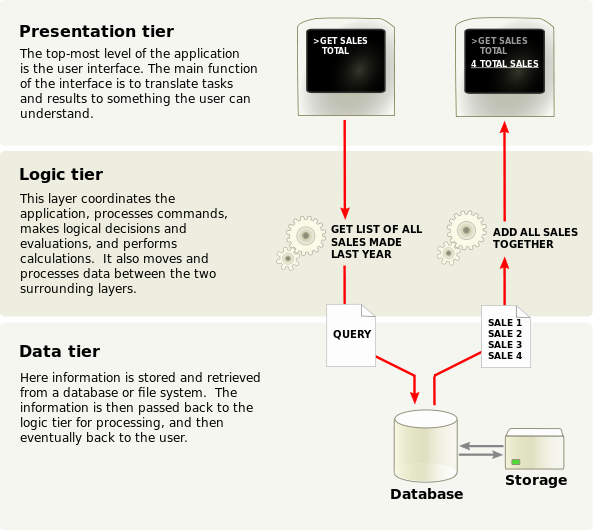
\includegraphics[width=0.6\textwidth]{assets/diagrams/3-tier-architecture.png}
	\caption{Schema architettura web 3-tier}
	\label{fig:3-tier-architecture}
\end{figure}

Questa tipologia di architettura garantisce maggiore scalabilità e manutenibilità,
in quanto qualunque modulo può essere aggiornato o sostituito indipendentemente
dal cambiamento di requisiti o tecnologie.


\section{Sessione utente}
Trattandosi di una piattaforma web le cui funzionalità sono pensate per essere
accessibili solo a seguito di autenticazione, la gestione della sessione utente
ne è una parte molto importante. Una sessione rappresenta infatti la possibilità
che un utente possa usufruire di un servizio in maniera continua, senza doversi
autenticare ad ogni operazione che necessita di verificare che si sia in possesso
di un account valido o che si abbiano permessi sufficienti.

\paragraph{Approccio basato su token}
L'approccio utilizzato è quello basato su \textbf{token}, per cui a seguito
di ogni autenticazione deve essere generato e associato all'utente un codice
univoco, volto a verificare la sessione. Questo codice, detto \textit{token}, è
definito come valido per un breve periodo di tempo, ma viene "rinnovato" ad ogni
richiesta effettuata dal client verso l'Application tier, così da garantire la
continuità della sessione, fino alla scadenza o al logout esplicito da parte
dell'utente.
Per ogni richiesta effettuate viene quindi verificato che l'utente sia autenticato
e che sia autorizzato ad effettuare eventuali operazioni riservate (ad esempio
accedere al pannello di amministrazione).


\section{Diagramma ER}

\begin{wrapfigure}{r}{0.4\textwidth}
	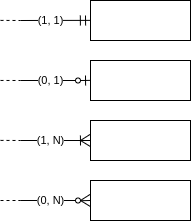
\includegraphics[width=\linewidth]{assets/diagrams/crows-foot-notation.png}
	\cprotect\caption{notazione \textit{crow's foot}}
	\label{fig:crows-foot-notation}
\end{wrapfigure}

Il diagramma in \autoref{fig:er-diagram} è stato progettato con MySQL WorkBench
\cite{workbench:9-EER} ed utilizza la notazione \textit{crow's foot}
\cite{wiki:crows-foot}, più orientata all'implementazione, in cui le relazioni
sono rappresentate da linee che collegano le entità e la cui cardinalità è
espressa tramite i simboli presenti alle estremità (\autoref{fig:crows-foot-notation}).

%%%%%%%%%%%%%%%%%%%%
{\color{red}\textbf{[\dots]}}
%%%%%%%%%%%%%%%%%%%%

\begin{figure}[ht]
	\centering
	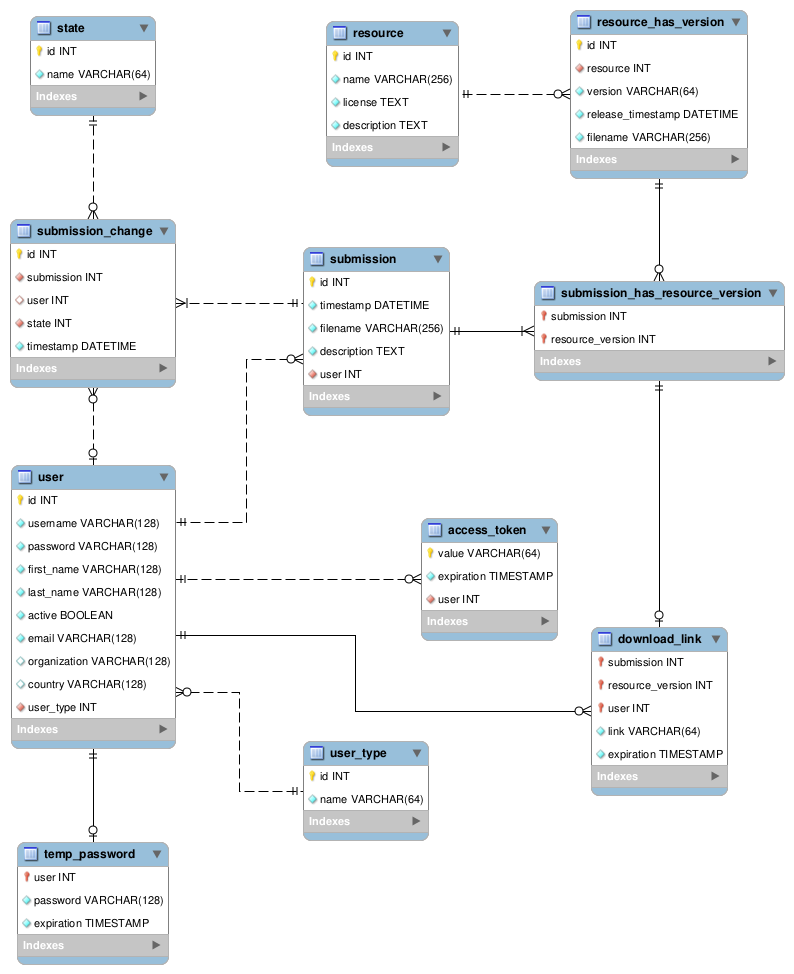
\includegraphics[width=\textwidth]{assets/diagrams/db-er-diagram.png}
	\caption{Diagramma ER}
	\label{fig:er-diagram}
\end{figure}